\documentclass{article}
%\usepackage{tex4ht}
\usepackage{amsmath}
\usepackage{amsfonts}
\usepackage{amssymb}
\usepackage{amsthm}
\usepackage{graphicx}
\usepackage{color}
\usepackage{float}
\usepackage{dsfont}
\setlength{\parskip}{0.5\baselineskip}
\author{Zhuo Liu (0983311)}
\title{Project on Automatic Learning (Phase 2, Part 1)}
\date{February 19, 2014}

\definecolor{lightgray}{gray}{0.5}


\begin{document}
\maketitle


\section{Introduction}

In this report, we will do the regular PCA on the data sets introduced in phase 1. The eigenvalues of the covariance matrices will be showed, and
samples in each data set will be projected into the space spanned by 2 principle components, so that data can be visulized.

%%% ------------------------------------------------------------------------------
\goodbreak

\section{Database: the Large One}

The data for this set is well distributed (i.e. no significant difference between different descriptors), so we will no standalize the data. We will
only consider the covariance matrix. Since there are 256 descriptors for this data set, it is impossible to list all the eigenvalues for covariance
matrix, we will have a summary on the eigenvalues (for the cumulative proportion on the trace):

 \begin{tabular}{|c|c|c|c|c|c|}
  \hline
                        & Comp.1 & Comp.2 & Comp.3 & Comp.4 & Comp.5 \\ \hline
  Cum. Prop. & 0.078 & 0.145 & 0.201 & 0.248 & 0.285 \\ \hline
                        & Comp.15 & Comp.24 & Comp.36 & Comp.59 & Comp.110 \\ \hline
  Cum. Prop. & 0.502 & 0.610 & 0.701 & 0.802 & 0.901 \\ \hline
 \end{tabular}
 
Therefore, in order to keep 80 percent energy, we have to keep at least 59 components as principle components.

Figure 1 shows the projection of obeservations into 2D PC space (different colors represent different classes).

\begin{figure}[htp]
\centering
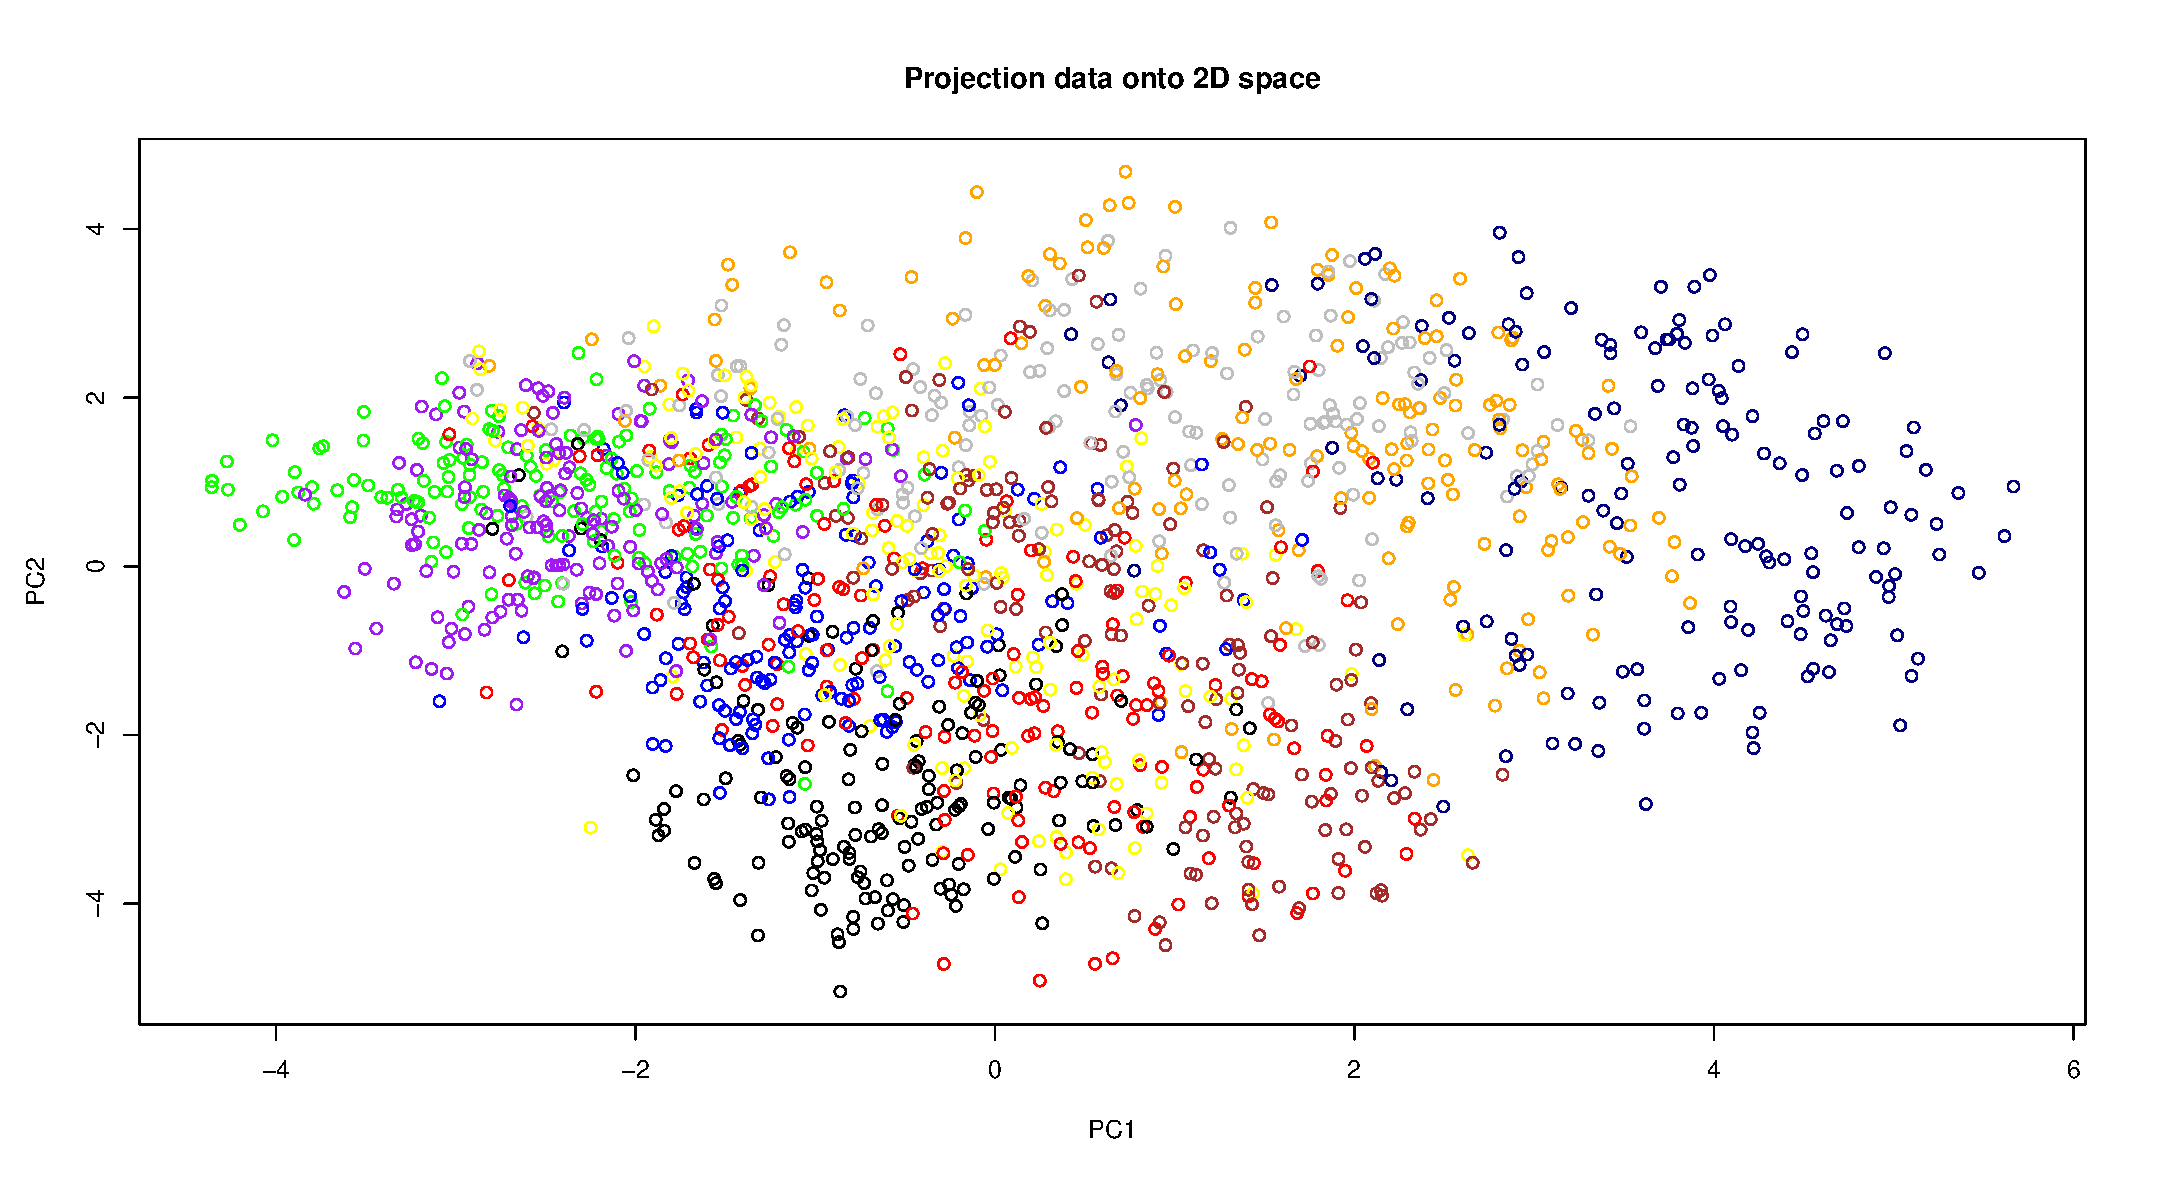
\includegraphics[width=12.1cm]{large_pca_projection_2D.eps}
\caption{Projection onto 2D principle components space.}
\end{figure}


%%% ------------------------------------------------------------------------------
\goodbreak

\section{Database: the Small One}

We will first check the PCA based on covariance matrix (i.e. data are not standalized), then we will check the result from correlation matrix (each
descriptor is standalized by dividing the standard deviation).

The eigenvalues for the covariance matrix is:

 \begin{tabular}{|c|c|c|c|c|c|}
  \hline
  Comp.1 & Comp.2 & Comp.3 & Comp.4 & Comp.5 & Comp.6 \\ \hline
  9.14e+03 & 5.32e+03 & 4.73e+03 & 2.28e+03 & 7.40e+02 & 2.27e+02 \\ \hline
  Comp.7 & Comp.8 & Comp.9 & Comp.10 & Comp.11 & Comp.12 \\ \hline
  5.66e+01 & 7.75e+00 & 3.02e+00 & 1.36e+00 & 2.57e-01 & 2.05e-02 \\ \hline
  Comp.13 & Comp.14 & Comp.15 & Comp.16 & Comp.17 & Comp.18 \\ \hline
  1.56e-03 & 5.19e-04 & 2.96e-12 & 1.98e-12 & 1.93e-12 & 1.67e-12 \\ \hline
  Comp.19 & & & & & \\ \hline
  5.96e-13 & & & & & \\ \hline
 \end{tabular}
 
If we want to keep at leat 90 percent energy, then we only need to keep the first four components as principle components, the corresponding 
proportion is:
\begin{equation}
 \frac{\sum_{k=1}^{4}\lambda_{k}}{\sum_{k=1}^{19}\lambda_{k}} = 0.9539754
\end{equation}

The following graph is the projection of observations into 2D principle components space.

\begin{figure}[htp]
\centering
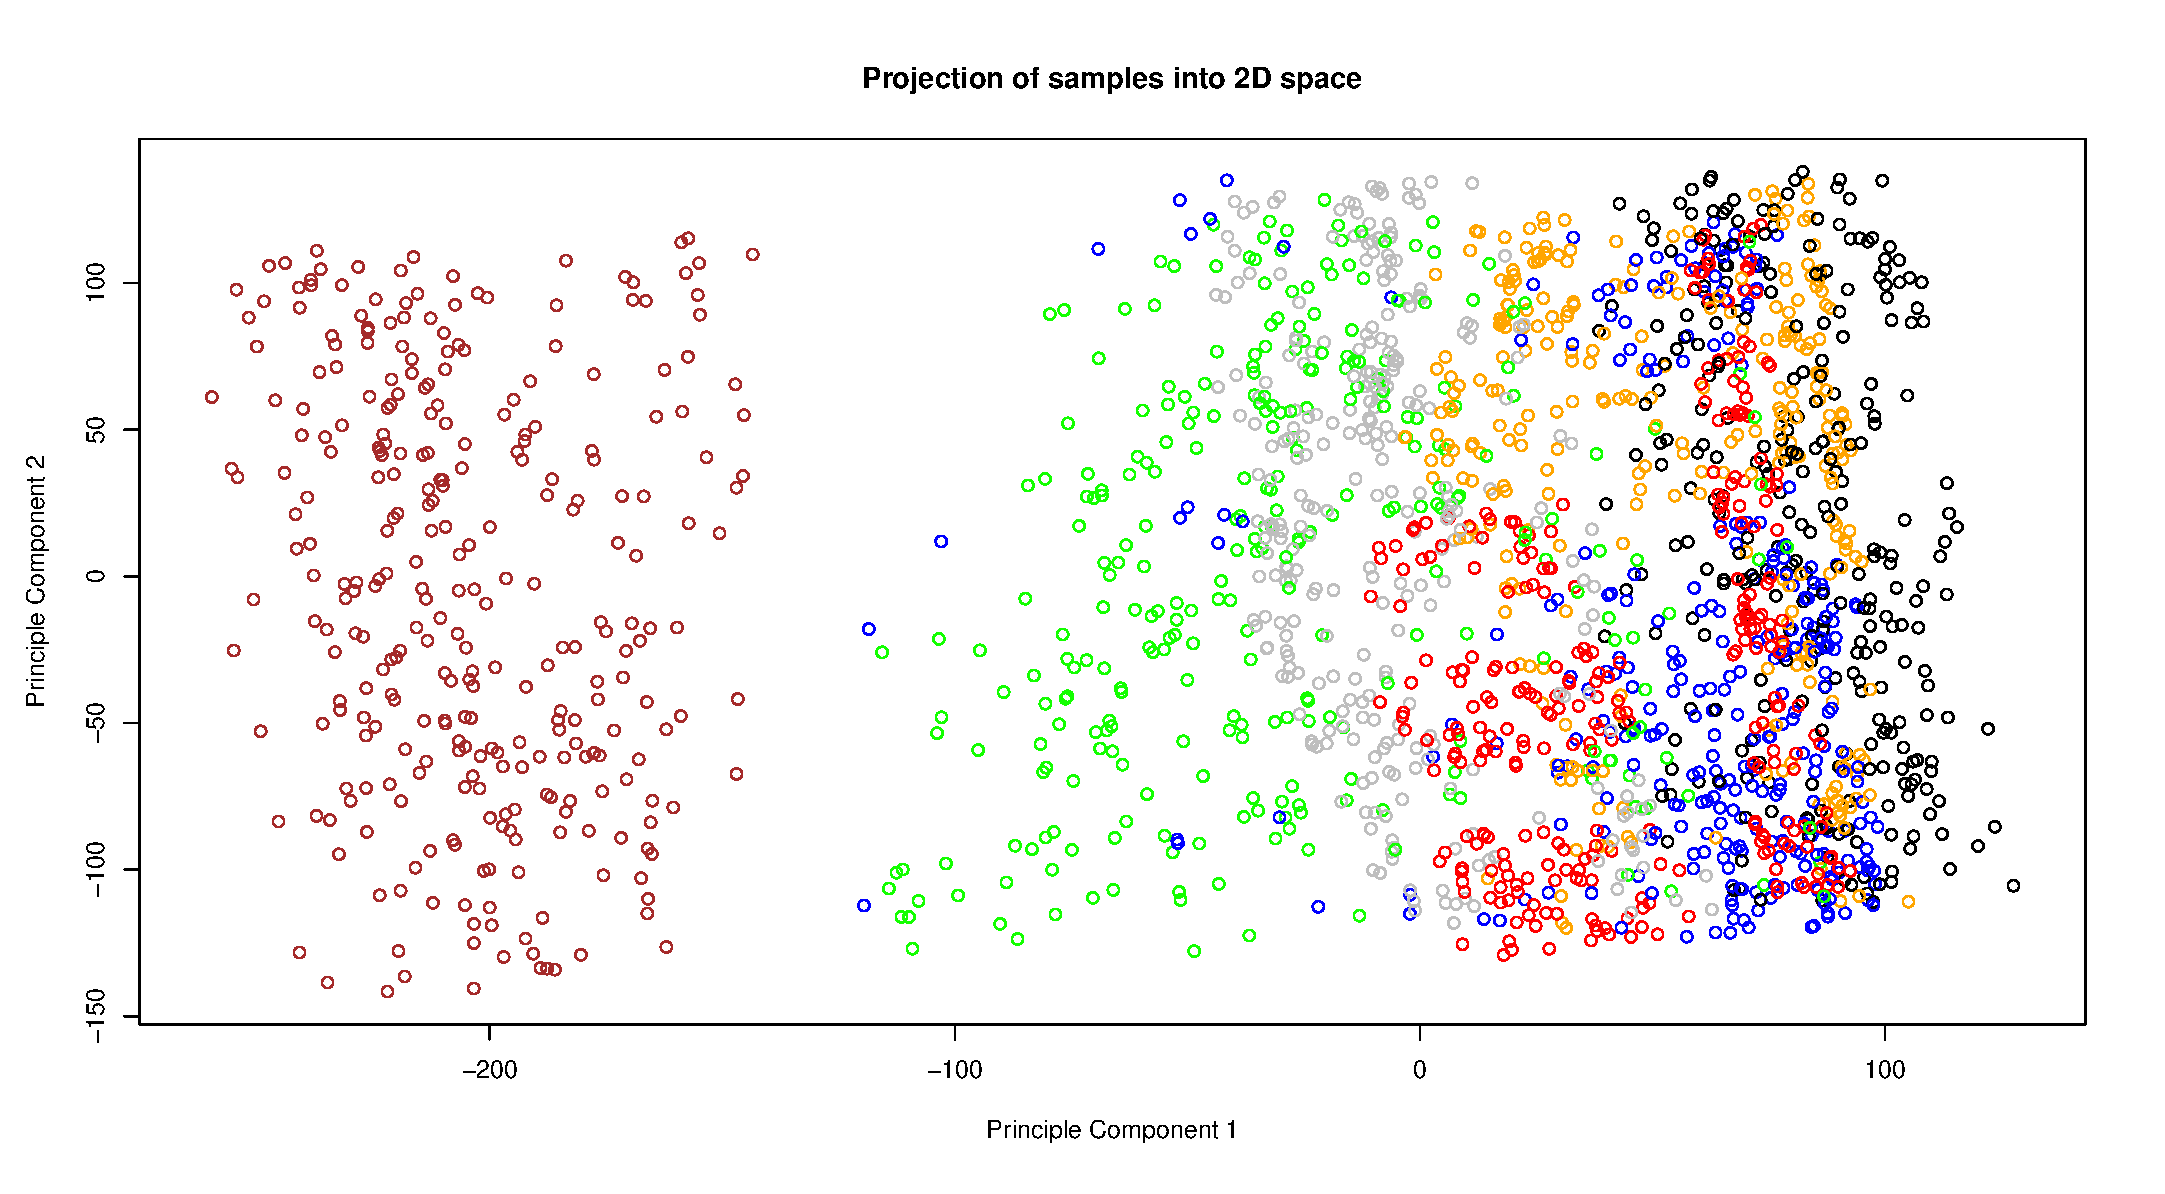
\includegraphics[width=12.1cm]{small_pca_projection_2D.eps}
\caption{Projection onto 2D principle components space. Here, the colors represent different classes: red--brickface, brown--sky, blue--foliage,
green--cement, orange--window, grey--path, black--grass.}
\end{figure}

Next, we will see what will happen if we consider the correlation matrix. Here, the descriptor ``pixel'' is a constant, in order to standalize
the data, we will remove this descriptor, otherwise, there will be some troubles. The following table shows the eigenvalues for the correlation
matrix:

 \begin{tabular}{|c|c|c|c|c|c|}
  \hline
  Comp.1 & Comp.2 & Comp.3 & Comp.4 & Comp.5 & Comp.6 \\ \hline
  7.62e+00 & 2.92e+00 & 1.79e+00 & 1.05e+00 & 9.35e-01 & 9.09e-01 \\ \hline
  Comp.7 & Comp.8 & Comp.9 & Comp.10 & Comp.11 & Comp.12 \\ \hline
  7.27e-01 & 5.62e-01 & 5.40e-01 & 3.95e-01 & 2.56e-01 & 1.79e-01 \\ \hline
  Comp.13 & Comp.14 & Comp.15 & Comp.16 & Comp.17 & Comp.18 \\ \hline
  1.11e-01 & 3.13e-04 & 2.58e-15 & 2.34e-15 & 2.32e-15 & 2.10e-15 \\ \hline
 \end{tabular}
 
If we want to keep at leat 90 percent energy, now we need to keep the first eight components as principle components, the corresponding 
proportion is:
\begin{equation}
 \frac{\sum_{k=1}^{8}\lambda_{k}}{\sum_{k=1}^{18}\lambda_{k}} = 0.91771445
\end{equation}

The projection onto the space spanned by first 2 PC is:

\begin{figure}[htp]
\centering
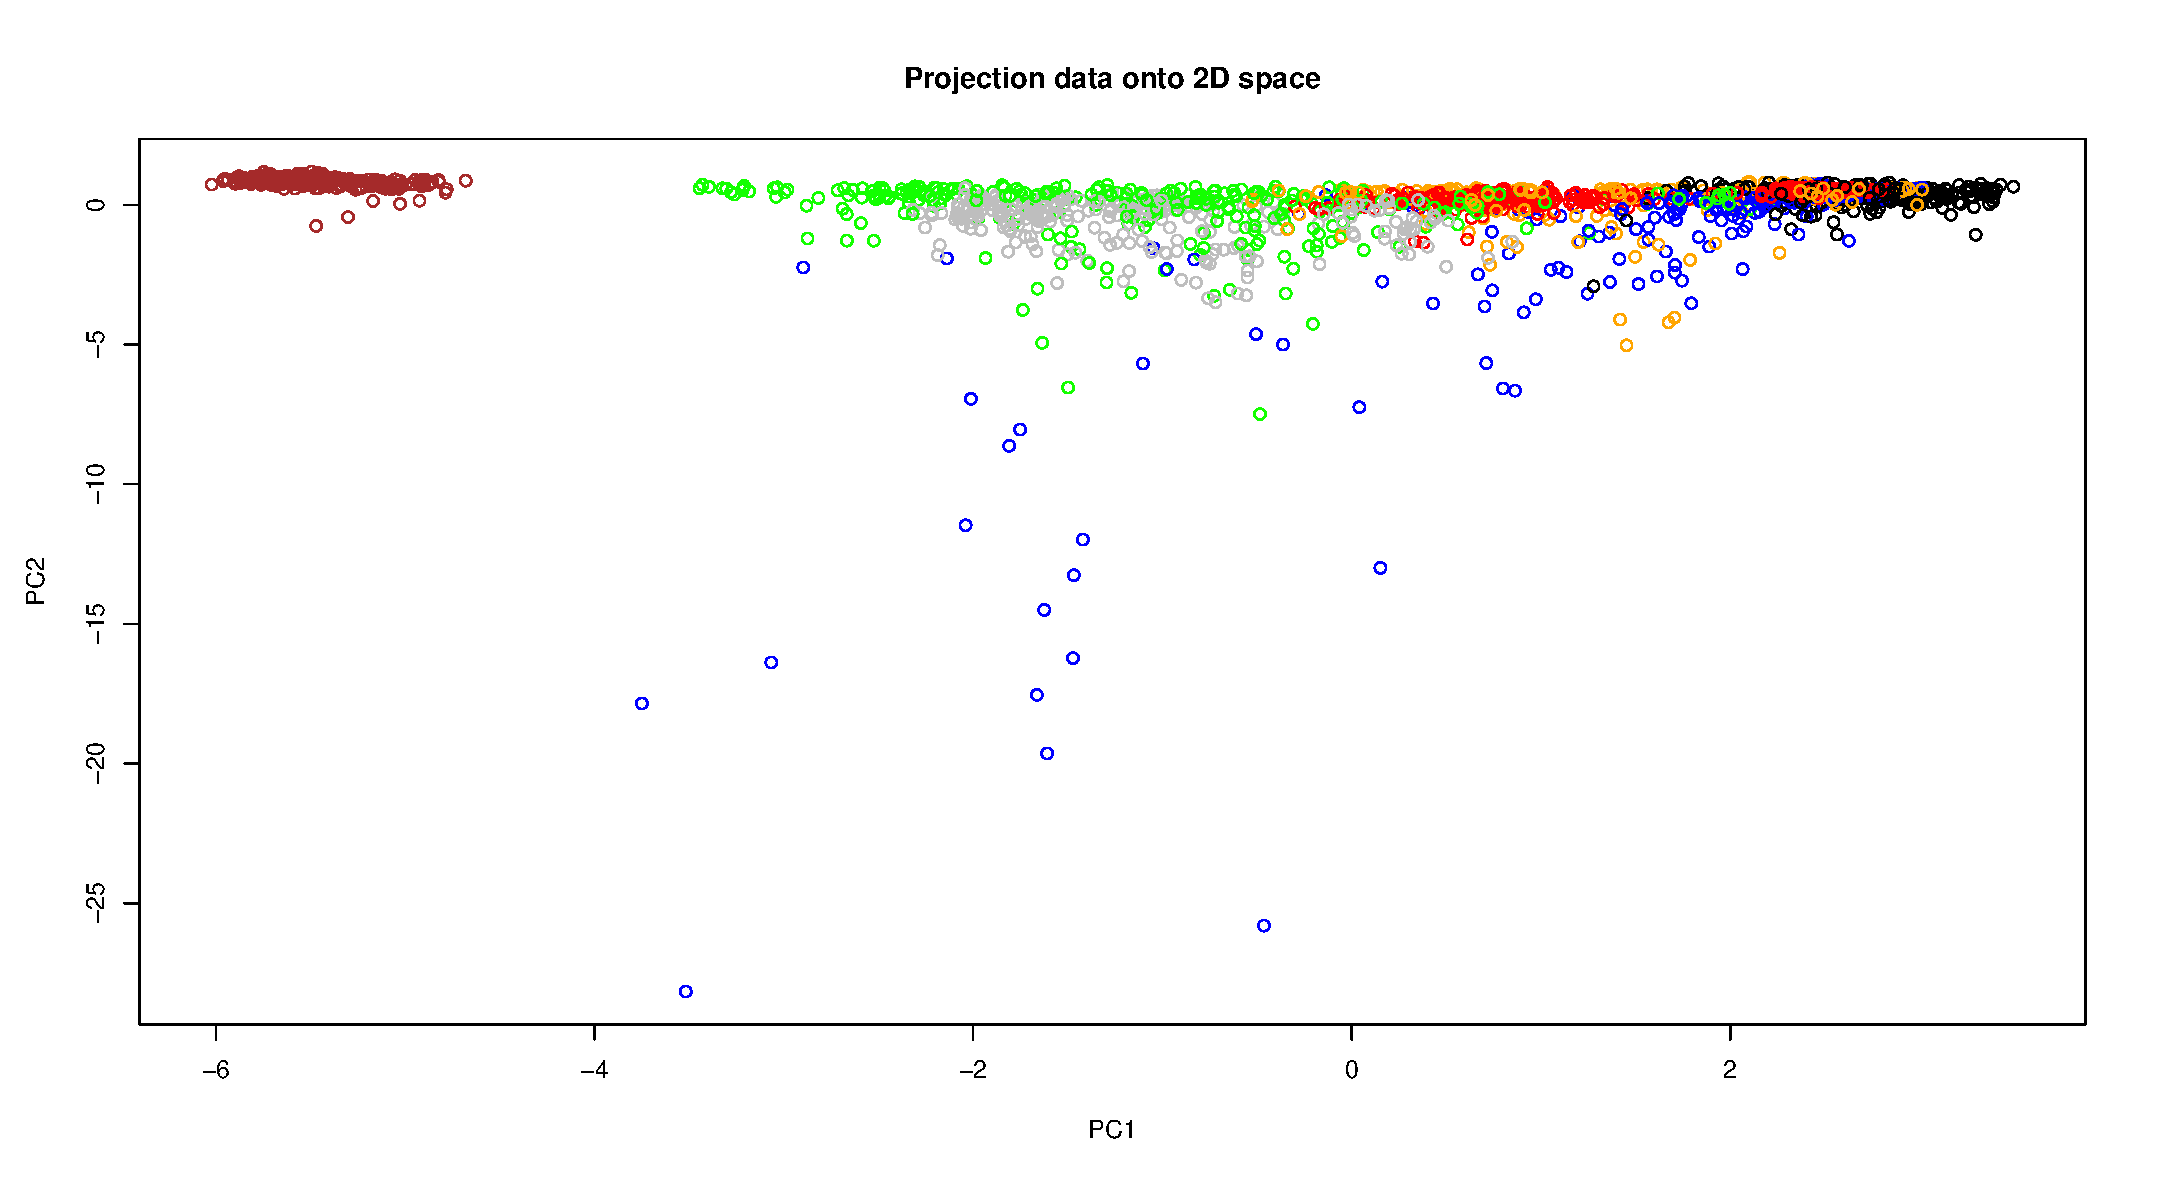
\includegraphics[width=12.1cm]{small_pca_projection_2D_2.eps}
\caption{Projection onto 2D principle components space. Here, the colors represent different classes: red--brickface, brown--sky, blue--foliage,
green--cement, orange--window, grey--path, black--grass.}
\end{figure}

\end{document}


